% Velotaf — Cover Design System
% Compile with: xelatex design-system-velotaf.tex
\documentclass[a4paper,11pt]{article}

\usepackage[margin=2.2cm]{geometry}
\usepackage{fontspec}
\usepackage{xcolor}
\usepackage{tikz}
\usepackage{tcolorbox}
\usepackage{graphicx}
\usepackage{tabularx}
\usepackage{booktabs}
\usepackage{colortbl}
\usepackage{pifont}
\usepackage{enumitem}
\usepackage{titlesec}
\usepackage[hidelinks]{hyperref}
\usepackage{fancyhdr}
\usepackage{parskip}
\usepackage{multicol}

\tcbuselibrary{skins,breakable}
\usetikzlibrary{shadows}

% ─── Fonts ───
\setmainfont{Avenir Next}[
  UprightFont = * Regular,
  BoldFont = * Bold,
  ItalicFont = * Italic,
  BoldItalicFont = * Bold Italic,
]
\setsansfont{Avenir Next}
\setmonofont{Menlo}
\newcommand{\knewave}{\fontspec{Marker Felt}}

% ─── Colors ───
\definecolor{veloRed}{HTML}{FF3232}
\definecolor{veloOrange}{HTML}{FF8F4D}
\definecolor{veloRedOrig}{HTML}{E94B35}
\definecolor{veloLightOrange}{HTML}{F06A42}
\definecolor{veloNavy}{HTML}{2E4057}
\definecolor{veloGold}{HTML}{F5A623}
\definecolor{veloWarm}{HTML}{F5F0EB}
\definecolor{veloDark}{HTML}{1A1A1A}
\definecolor{veloText}{HTML}{2D2D2D}
\definecolor{bleenGreen}{HTML}{00C48C}
\definecolor{pageBg}{HTML}{FAFAF8}
\definecolor{cardBg}{HTML}{FFFFFF}
\definecolor{grayLight}{HTML}{F3F4F6}
\definecolor{grayMid}{HTML}{9CA3AF}
\definecolor{grayDark}{HTML}{4B5563}

\pagecolor{pageBg}

% ─── Table styling ───
\definecolor{tableHeader}{HTML}{F0F0F0}
\definecolor{tableRowAlt}{HTML}{F8F8F6}
\newcommand{\tableheader}{\rowcolor{tableHeader}\bfseries}

% ─── Header/Footer ───
\pagestyle{fancy}
\fancyhf{}
\renewcommand{\headrulewidth}{0pt}
\fancyfoot[L]{\small\color{grayMid}Velotaf Design System — Denis Henin · uixbydenis.eu}
\fancyfoot[R]{\small\color{grayMid}\thepage}

% ─── Custom commands ───
\newcommand{\colorswatch}[3]{%
  \begin{tikzpicture}
    \fill[#1, rounded corners=4pt] (0,0) rectangle (1.2,1.2);
    \node[anchor=west, font=\small\bfseries, text=veloText] at (1.45,0.75) {#2};
    \node[anchor=west, font=\footnotesize\ttfamily, text=grayMid] at (1.45,0.35) {#3};
  \end{tikzpicture}%
}

\newcommand{\sectionrule}{%
  \vspace{4pt}%
  \noindent
\begin{tikzpicture}
    \shade[left color=veloRed, right color=veloOrange] (0,0) rectangle (\textwidth, 2.5pt);
  \end{tikzpicture}%
  \vspace{6pt}%
}

% ─── Section title formatting ───
\titleformat{\section}
  {\fontsize{22}{26}\selectfont\bfseries\sffamily\color{veloText}}
  {\thesection.}{0.5em}{}
\titleformat{\subsection}
  {\fontsize{14}{18}\selectfont\bfseries\sffamily\color{veloText}}
  {\thesubsection}{0.5em}{}

\newcommand{\tagpill}[2]{%
  \tikz[baseline=(tag.base)]{%
    \node[fill=#1, text=white, rounded corners=3pt, inner sep=3pt, font=\tiny\bfseries] (tag) {#2};%
  }%
}

% ─── tcolorbox styles ───
\tcbset{
  card/.style={
    enhanced,
    colback=cardBg,
    colframe=grayLight,
    boxrule=0.4pt,
    arc=6pt,
    left=12pt, right=12pt, top=10pt, bottom=10pt,
    fonttitle=\bfseries\sffamily,
    coltitle=veloText,
    drop shadow={shadow xshift=0.5pt, shadow yshift=-1.5pt, opacity=0.12},
    breakable,
  },
  highlight card/.style={
    card,
    borderline north={2pt}{0pt}{veloRed!70!veloOrange},
  }
}

% ─── Do/Don't icons ───
\newcommand{\doitem}[1]{\item[\textcolor{bleenGreen}{\ding{51}}] #1}
\newcommand{\dontitem}[1]{\item[\textcolor{veloRed}{\ding{55}}] #1}

\begin{document}

% ═══════════════════════════════════════════
% TITLE PAGE
% ═══════════════════════════════════════════

\thispagestyle{empty}

\begin{tikzpicture}[remember picture, overlay]
  % Background gradient
  \shade[left color=veloRed, right color=veloOrange]
    (current page.north west) rectangle ([yshift=-9cm]current page.north east);
  % Dark bottom
  \fill[veloDark]
    ([yshift=-9cm]current page.north west) rectangle (current page.south east);
\end{tikzpicture}

\vspace*{0.8cm}

\begin{center}
  
\includegraphics[width=9cm]{../covers/layers/cover-1-text.png}\\[6pt]
  {\Large\color{white}\bfseries Cover Art — Design System}\\[4pt]
  {\small\color{white!60}Version 1.0 — Mars 2026}\\[2pt]
  {\small\color{white!40}Denis Henin — Graphiste Designer @ bleen}
\end{center}

\vspace{0.4cm}

\begin{center}
  \begin{tikzpicture}
    \node[drop shadow={shadow xshift=1pt, shadow yshift=-2pt, opacity=0.3, fill=black}, inner sep=0pt] {%
      \includegraphics[width=7.5cm]{../covers/cover-1-pure.png}%
    };
  \end{tikzpicture}
\end{center}

\vfill

\begin{center}
  {\footnotesize\color{white!30}Cover « Pure — Gradient Original » · 3000×3000px}
\end{center}

\newpage

% ═══════════════════════════════════════════
% TABLE OF CONTENTS
% ═══════════════════════════════════════════

\tableofcontents
\newpage

% ═══════════════════════════════════════════
% 1. CONTEXTE
% ═══════════════════════════════════════════

\section{Contexte du podcast}
\sectionrule

\begin{tcolorbox}[card]
\rowcolors{2}{white}{tableRowAlt}
\begin{tabularx}{\textwidth}{@{}lX@{}}
\toprule
\tableheader Élément & Détail \\
\midrule
Nom & Vélotaf \\
Tagline & « Le vélo n'est pas un simple objet » \\
Format & Interview mensuel, 25--55 min, 102+ épisodes, 3 saisons \\
Host & Victor Blanchard (animateur), Olivier De Schutter (créateur) \\
Producteur & bleen \\
Origine & Mouvement Two Wheel Tuesday (2WT), reconnu par le WEF \\
Notes & 4.9/5 Apple Podcasts · 4.8/5 Spotify \\
Audience & Vélotafeurs francophones (FR + BE), urbains, sensibilité écolo \\
Thèmes & Mobilité douce, urbanisme, inégalités, écologie, société \\
\bottomrule
\end{tabularx}
\end{tcolorbox}

\subsection{Positionnement}

Pas un podcast sportif/performance. C'est un \textbf{podcast sociétal} qui utilise le vélo comme prisme pour parler urbanisme, écologie, inclusivité, rapport au temps et à l'espace. Ton engagé mais accessible, ni militant ni culpabilisant.

\subsection{Ce que la marque est}

\begin{itemize}[nosep]
  \item Chaleureuse, énergique, concrète
  \item Un mec normal sur son vélo, pas un athlète
  \item Le vélo comme prisme sur la société
  \item Optimiste mais lucide
  \item Engagé sans être donneur de leçons
\end{itemize}

\subsection{Ce que la marque n'est pas}

\begin{itemize}[nosep]
  \item Sportif/performance (pas de lycra, pas de chrono)
  \item Militant agressif/culpabilisant
  \item Corporate/froid
  \item Minimaliste/austère
  \item Élitiste
\end{itemize}

\newpage

% ═══════════════════════════════════════════
% 2. PALETTE DE COULEURS
% ═══════════════════════════════════════════

\section{Palette de couleurs}
\sectionrule

\subsection{Gradient de la cover}

Le fond de la cover utilise un \textbf{dégradé horizontal} (gauche → droite), fidèle à la cover originale du podcast.

\begin{tcolorbox}[card]
\begin{center}
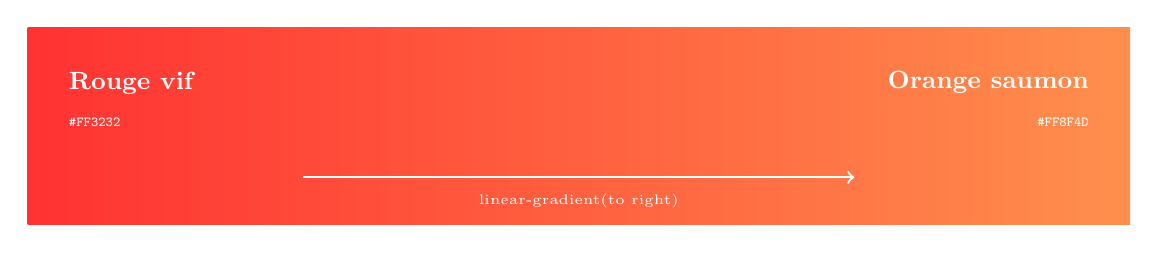
\begin{tikzpicture}
  \shade[left color=veloRed, right color=veloOrange] (0,0) rectangle (14,2.5);
  \node[font=\small\bfseries, text=white, anchor=west] at (0.4, 1.8) {Rouge vif};
  \node[font=\tiny\ttfamily, text=white, anchor=west] at (0.4, 1.3) {\#FF3232};
  \node[font=\small\bfseries, text=white, anchor=east] at (13.6, 1.8) {Orange saumon};
  \node[font=\tiny\ttfamily, text=white, anchor=east] at (13.6, 1.3) {\#FF8F4D};
  \draw[white, thick, ->] (3.5, 0.6) -- (10.5, 0.6);
  \node[font=\tiny, text=white] at (7, 0.3) {linear-gradient(to right)};
\end{tikzpicture}
\end{center}
\end{tcolorbox}

\begin{verbatim}
CSS: background: linear-gradient(to right, #FF3232, #FF8F4D);
\end{verbatim}

\subsection{Couleurs principales}

\noindent
\colorswatch{veloRed}{Rouge vif}{\#FF3232}\hspace{18pt}%
\colorswatch{veloOrange}{Orange saumon}{\#FF8F4D}\hspace{18pt}%
\colorswatch{veloRedOrig}{Red-Orange orig.}{\#E94B35}

\vspace{6pt}\noindent
\colorswatch{veloLightOrange}{Light Orange}{\#F06A42}\hspace{18pt}%
\colorswatch{white}{Blanc}{\#FFFFFF}\hspace{18pt}%
\colorswatch{veloText}{Noir doux}{\#2D2D2D}

\subsection{Couleurs secondaires}

\noindent
\colorswatch{veloNavy}{Bleu marine}{\#2E4057}\hspace{18pt}%
\colorswatch{veloGold}{Gold doré}{\#F5A623}\hspace{18pt}%
\colorswatch{veloWarm}{Crème chaud}{\#F5F0EB}\hspace{18pt}%
\colorswatch{veloDark}{Anthracite}{\#1A1A1A}

\subsection{Règles d'utilisation}

\begin{tcolorbox}[highlight card, title=Ratio 60-30-10]
\begin{itemize}[nosep]
  \item \textbf{60\%} — Gradient rouge-orange (fond dominant)
  \item \textbf{30\%} — Blanc pour la typographie et l'air
  \item \textbf{10\%} — Accents (bleu marine, gold, ou ombres)
\end{itemize}
\end{tcolorbox}

\begin{tcolorbox}[card, title=Interdits, colframe=veloRed!30]
\begin{itemize}[nosep]
  \item Pas de gris moyen (\#888, \#999) — la palette est franche
  \item Pas de pastels — saturation $>$ 30\%
  \item Pas de noir pur (\#000000) — utiliser \texttt{\#2D2D2D} ou \texttt{\#1A1A1A}
  \item Pas de bleu électrique ou vert fluo
\end{itemize}
\end{tcolorbox}

\newpage

% ═══════════════════════════════════════════
% 3. TYPOGRAPHIE
% ═══════════════════════════════════════════

\section{Typographie}
\sectionrule

\subsection{Logo « VÉLOTAF »}

\begin{tcolorbox}[card]
\begin{center}
\includegraphics[width=\linewidth]{../covers/cover-1-pure.png}
\end{center}

\vspace{6pt}

\begin{tabularx}{\textwidth}{@{}lX@{}}
\toprule
\textbf{Propriété} & \textbf{Valeur} \\
\midrule
Police & Knewave (Google Fonts) \\
Style & Cursive / brush, tout en majuscules \\
Couleur & Blanc pur sur fond gradient \\
Stroke & Contour noir semi-transparent (4px, opacité 0.7) \\
Ombre & Text-shadow noir multi-directionnel + glow \\
Effet & Chaque lettre légèrement rotée (±1--2°) et décalée verticalement \\
Accent & Le « É » porte un accent aigu — ne jamais l'oublier \\
\bottomrule
\end{tabularx}
\end{tcolorbox}

\subsection{Hiérarchie typographique}

\begin{tcolorbox}[card]
\rowcolors{2}{white}{tableRowAlt}
\begin{tabularx}{\textwidth}{@{}llXl@{}}
\toprule
\tableheader Usage & Police & Justification & Taille \\
\midrule
Logo / Titre & Knewave & Énergie, caractère urbain & 750px (export 3k) \\
Sous-titres & Plus Jakarta Sans Bold & Lisibilité, modernité & 24--32pt \\
Corps & Plus Jakarta Sans Regular & Neutralité, confort & 14--18pt \\
Accents & Caveat, Patrick Hand & Rappel du côté manuscrit & variable \\
\bottomrule
\end{tabularx}
\end{tcolorbox}

\subsection{Traitement du texte sur la cover}

Le titre est traité avec plusieurs couches d'effets pour assurer la lisibilité sur le gradient :

\begin{enumerate}[nosep]
  \item \textbf{Remplissage} : blanc pur \texttt{\#FFFFFF}
  \item \textbf{Contour (stroke)} : noir à 70\% d'opacité, 26px d'épaisseur (à l'échelle 3000px)
  \item \textbf{Paint-order} : \texttt{stroke fill} — le contour est peint sous le remplissage
  \item \textbf{Ombres} : 4 ombres directionnelles (±3px) + 1 ombre douce (16px blur)
  \item \textbf{Animation typographique} : chaque lettre a une rotation et un décalage vertical aléatoire
\end{enumerate}

\newpage

% ═══════════════════════════════════════════
% 4. ILLUSTRATION
% ═══════════════════════════════════════════

\section{Illustration}
\sectionrule

\subsection{Style}

\begin{tcolorbox}[card]
\begin{tabularx}{\textwidth}{@{}lX@{}}
\toprule
\textbf{Propriété} & \textbf{Description} \\
\midrule
Type & Illustration vectorielle flat design \\
Rendu & Semi-réaliste, stylisé (pas cartoon, pas photo-réaliste) \\
Traits & Contours nets, pas de ligne noire visible (formes pleines) \\
Ombres & Minimales, par aplats de couleur plus sombre \\
Détails & Suffisamment détaillés pour être reconnaissable \\
Perspective & Vue de face, légère contre-plongée \\
\bottomrule
\end{tabularx}
\end{tcolorbox}

\subsection{Personnage}

\begin{itemize}[nosep]
  \item Homme barbu à lunettes de soleil, casque vélo
  \item Style urbain-chic : blazer bleu + chemise blanche
  \item Position : sur un vélo, mains sur le guidon, en mouvement
  \item Le personnage est l'élément central — il occupe $\sim$60\% de la hauteur
  \item Expression souriante, décontractée
\end{itemize}

\subsection{Fichier source}

\begin{tcolorbox}[card]
\begin{tabularx}{\textwidth}{@{}lX@{}}
\toprule
\textbf{Fichier} & \textbf{Détail} \\
\midrule
\texttt{velotaf\_backup.png} & Image source (nobg, fond transparent) \\
Dimensions & 1028 × 932 px \\
Format & PNG RGBA \\
Placement & \texttt{width:132\%; left:-22\%; bottom:-8px} (à l'échelle 3000px) \\
Filtre & Drop-shadow léger (0.3 / 0.15 opacité) \\
\bottomrule
\end{tabularx}
\end{tcolorbox}

\newpage

% ═══════════════════════════════════════════
% 5. COMPOSITION
% ═══════════════════════════════════════════

\section{Composition \& mise en page}
\sectionrule

\subsection{Structure de la cover (3000×3000px)}

\begin{tcolorbox}[card]
\begin{center}
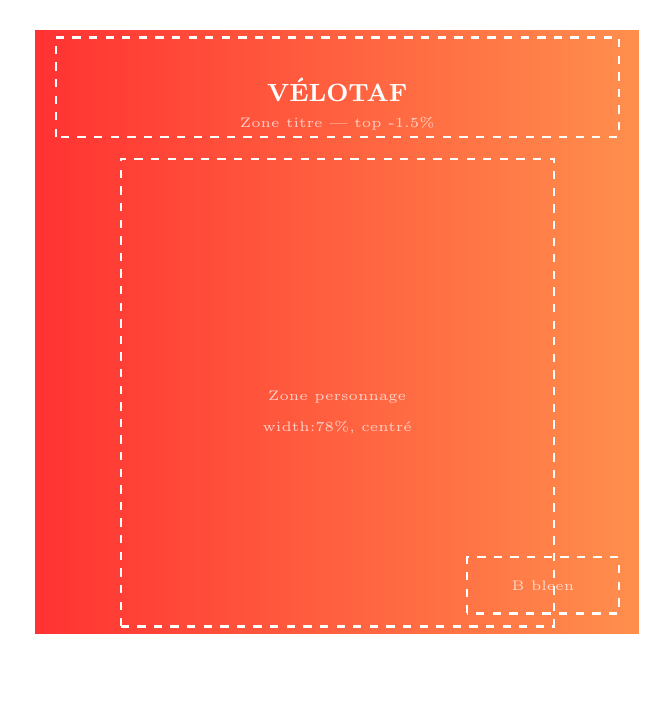
\begin{tikzpicture}[scale=0.55]
  % Cover frame
  \shade[left color=veloRed, right color=veloOrange] (0,0) rectangle (14,14);
  \draw[white, thick] (0,0) rectangle (14,14);

  % Title zone
  \draw[white, dashed, thick] (0.5,11.5) rectangle (13.5,13.8);
  \node[font=\small\bfseries, text=white] at (7,12.6) {VÉLOTAF};
  \node[font=\tiny, text=white, opacity=0.7] at (7,11.8) {Zone titre — top -1.5\%};

  % Character zone
  \draw[white, dashed, thick] (2,0.2) rectangle (12,11);
  \node[font=\tiny, text=white, opacity=0.7] at (7,5.5) {Zone personnage};
  \node[font=\tiny, text=white, opacity=0.7] at (7,4.8) {width:78\%, centré};

  % Logo zone
  \draw[white, dashed, thick] (10,0.5) rectangle (13.5,1.8);
  \node[font=\tiny, text=white, opacity=0.7] at (11.75,1.15) {B bleen};

  % Margins
  \draw[white!50, <->] (0,-0.5) -- (0.7,-0.5);
  \node[font=\tiny, text=white!50, anchor=north] at (0.35,-0.5) {5\%};
\end{tikzpicture}
\end{center}
\end{tcolorbox}

\subsection{Règles de composition}

\begin{itemize}[nosep]
  \item \textbf{Titre en haut} : toujours au-dessus du personnage, jamais derrière
  \item \textbf{Personnage centré} : point focal, regard vers le spectateur
  \item \textbf{Fond gradient} : pas de photo, pas de paysage — le gradient suffit
  \item \textbf{Espacement généreux} : le design respire, pas d'encombrement
  \item \textbf{Logo} : B bleen regroupés, discret, bas-droite
\end{itemize}

\subsection{Calques d'export}

Chaque cover est exportée en calques séparés (3000×3000px PNG) :

\begin{tcolorbox}[card]
\rowcolors{2}{white}{tableRowAlt}
\begin{tabularx}{\textwidth}{@{}llXl@{}}
\toprule
\tableheader Calque & Fichier & Contenu & Taille \\
\midrule
Background & \texttt{cover-1-bg.png} & Gradient + grain & 1.6 MB \\
Personnage & \texttt{cover-1-character.png} & Illustration, fond transparent & 1.8 MB \\
Texte & \texttt{cover-1-text.png} & « VÉLOTAF », fond transparent & 591 KB \\
Logo & \texttt{cover-1-logo.png} & B bleen, fond transparent & 68 KB \\
\midrule
Composite & \texttt{cover-1-pure.png} & Tous calques fusionnés & 3.6 MB \\
\bottomrule
\end{tabularx}
\end{tcolorbox}

\newpage

% ═══════════════════════════════════════════
% 6. LOGO BLEEN
% ═══════════════════════════════════════════

\section{Logo Bleen}
\sectionrule

\subsection{Composition du bloc logo}

Le logo sur la cover combine deux éléments SVG en un seul bloc :

\begin{tcolorbox}[card]
\begin{tabularx}{\textwidth}{@{}lX@{}}
\toprule
\textbf{Élément} & \textbf{Détail} \\
\midrule
Icône « B » & Forme double-bulle Bleen, viewBox 0 0 200 280 \\
Texte « bleen » & Logotype, viewBox 270 60 450 160 \\
Couleur & \texttt{rgba(255,255,255,0.6)} — blanc à 60\% d'opacité \\
Gap & 6px entre icône et texte (à l'échelle 3000px) \\
Position & \texttt{bottom:6\%; right:6\%} \\
Filtre & \texttt{drop-shadow(0 4px 8px rgba(0,0,0,0.2))} \\
\bottomrule
\end{tabularx}
\end{tcolorbox}

\subsection{Ratios du logo SVG (source : bleenconsulting.webflow.io)}

Proportions extraites du SVG officiel Bleen (viewBox \texttt{0 0 720 280}) :

\begin{tcolorbox}[card]
\begin{tabularx}{\textwidth}{@{}lX@{}}
\toprule
\textbf{Mesure} & \textbf{Valeur} \\
\midrule
ViewBox global & 720 $\times$ 280 (ratio 18:7 $\approx$ 2.57:1) \\
\midrule
\multicolumn{2}{@{}l}{\textit{Symbole « B »}} \\
Bounding box & x=0$\rightarrow$200, y=0$\rightarrow$280 — soit 200 $\times$ 280 (ratio 5:7) \\
Grand cercle & 200 $\times$ 200 (y=80$\rightarrow$280) \\
Petit cercle & 160 $\times$ 160 (y=0$\rightarrow$160) — ratio petit/grand = 4:5 \\
Chevauchement & 80 unités verticales (y=80$\rightarrow$160) \\
\midrule
\multicolumn{2}{@{}l}{\textit{Texte « bleen »}} \\
Bounding box & x=270$\rightarrow$720, y=70$\rightarrow$210 — soit 450 $\times$ 140 \\
\midrule
\multicolumn{2}{@{}l}{\textit{Rapports clés}} \\
Symbole : Gap : Texte (largeur) & 200 : 70 : 450 ($\approx$ 28\% : 10\% : 62\%) \\
Largeur symbole / largeur texte & 200/450 = 0.444 (le symbole fait 44\% du texte) \\
Hauteur symbole / hauteur texte & 280/140 = 2.0 (le symbole fait 2$\times$ la hauteur du texte) \\
\bottomrule
\end{tabularx}
\end{tcolorbox}

\subsection{Règles}

\begin{itemize}[nosep]
  \item Opacité réduite pour ne pas détourner l'attention du personnage
  \item Ombre légère pour la lisibilité sur fonds clairs et sombres
\end{itemize}

\newpage

% ═══════════════════════════════════════════
% 7. EFFETS & OVERLAYS
% ═══════════════════════════════════════════

\section{Effets \& overlays}
\sectionrule

La cover « Pure » est volontairement minimale en effets pour rester fidèle à la cover originale.

\begin{tcolorbox}[card]
\begin{tabularx}{\textwidth}{@{}llX@{}}
\toprule
\textbf{Effet} & \textbf{Intensité} & \textbf{Description} \\
\midrule
Grain & 3\% opacité & Texture de bruit fractal, blend mode overlay \\
Drop-shadow personnage & Léger & \texttt{0 1px 3px rgba(0,0,0,0.3)} + \texttt{0 6px 14px rgba(0,0,0,0.15)} \\
Text stroke & 26px & Contour noir à 70\% autour du titre \\
Text shadow & Multi & 4 directions + glow diffus \\
\bottomrule
\end{tabularx}
\end{tcolorbox}


\newpage

% ═══════════════════════════════════════════
% 8. SPECS TECHNIQUES
% ═══════════════════════════════════════════

\section{Spécifications techniques}
\sectionrule

\subsection{Format de la cover}

\begin{tcolorbox}[card]
\begin{tabularx}{\textwidth}{@{}lX@{}}
\toprule
\textbf{Propriété} & \textbf{Valeur} \\
\midrule
Dimensions & 3000 × 3000 px (carré) \\
Résolution & 72 DPI (optimisé écran) \\
Format & PNG 24-bit avec alpha (calques) / PNG opaque (composite) \\
Espace colorimétrique & sRGB \\
Poids composite & $\sim$3.6 MB \\
\bottomrule
\end{tabularx}
\end{tcolorbox}

\subsection{CSS de référence}

\begin{tcolorbox}[card, colback=veloDark, coltitle=white, coltext=white!90]
\begin{verbatim}
/* Gradient de fond */
background: linear-gradient(to right, #FF3232, #FF8F4D);

/* Personnage */
width: 132%;
left: -22%;
bottom: -70px;
filter: drop-shadow(0 1px 3px rgba(0,0,0,0.3))
        drop-shadow(0 6px 14px rgba(0,0,0,0.15));

/* Titre VELOTAF */
font-family: 'Knewave', cursive;
font-size: 750px;  /* @ 3000px */
color: white;
-webkit-text-stroke: 26px rgba(0,0,0,0.7);
paint-order: stroke fill;

/* Logo B bleen */
bottom: 6%; right: 6%;
color: rgba(255,255,255,0.6);
gap: 6px;
\end{verbatim}
\end{tcolorbox}

\newpage

% ═══════════════════════════════════════════
% 9. DÉCLINAISONS
% ═══════════════════════════════════════════

\section{Déclinaisons recommandées}
\sectionrule

\subsection{Formats réseaux sociaux}

\begin{tcolorbox}[card]
\rowcolors{2}{white}{tableRowAlt}
\begin{tabularx}{\textwidth}{@{}llX@{}}
\toprule
\tableheader Plateforme & Dimensions & Adaptation \\
\midrule
Instagram post & 1080 × 1080 & Cover art ou variante avec citation \\
Instagram story & 1080 × 1920 & Fond gradient, personnage en bas, titre épisode en haut \\
Bannière Twitter/X & 1500 × 500 & Personnage à gauche, titre + tagline à droite \\
Bannière LinkedIn & 1584 × 396 & Idem Twitter, adapté au format \\
Miniature YouTube & 1280 × 720 & Personnage + titre épisode en gros \\
\bottomrule
\end{tabularx}
\end{tcolorbox}

\subsection{Do's \& Don'ts}

\begin{multicols}{2}
\begin{tcolorbox}[card, title={\color{bleenGreen!80!black}Do's}, colframe=bleenGreen!30, borderline north={2pt}{0pt}{bleenGreen}]
\begin{itemize}[nosep, leftmargin=16pt]
  \doitem{Fond gradient comme élément dominant}
  \doitem{Typo Knewave uniquement pour le logo}
  \doitem{Décliner l'illustration dans le même style flat}
  \doitem{Garder le contraste blanc/gradient}
  \doitem{Ambiance décontractée et positive}
\end{itemize}
\end{tcolorbox}

\begin{tcolorbox}[card, title={\color{veloRed}Don'ts}, colframe=veloRed!30, borderline north={2pt}{0pt}{veloRed}]
\begin{itemize}[nosep, leftmargin=16pt]
  \dontitem{Photos en fond}
  \dontitem{Dégradés complexes ou effets 3D}
  \dontitem{Changer la couleur du fond signature}
  \dontitem{Logo en minuscules ou police standard}
  \dontitem{Surcharger les visuels}
  \dontitem{Noir pur \texttt{\#000000}}
\end{itemize}
\end{tcolorbox}
\end{multicols}

\vfill

\begin{center}

\begin{tikzpicture}
  \shade[left color=veloRed, right color=veloOrange] (0,0) rectangle (\textwidth, 2pt);
\end{tikzpicture}\\[8pt]
{\small\color{grayMid} Document généré le \today\ — Bleen Consulting}
\end{center}

\end{document}
